%package list
\documentclass{article}
\usepackage[top=3cm, bottom=3cm, outer=3cm, inner=3cm]{geometry}
\usepackage{multicol}
\usepackage{graphicx}
\usepackage{url}
%\usepackage{cite}
\usepackage{hyperref}
\usepackage{array}
%\usepackage{multicol}
\newcolumntype{x}[1]{>{\centering\arraybackslash\hspace{0pt}}p{#1}}
\usepackage{natbib}
\usepackage{pdfpages}
\usepackage{multirow}
\usepackage[utf8]{inputenc}
\usepackage[normalem]{ulem}
\useunder{\uline}{\ul}{}
\usepackage{svg}
\usepackage{xcolor}
\usepackage{listings}
\lstdefinestyle{ascii-tree}{
    literate={├}{|}1 {─}{--}1 {└}{+}1 
  }
\lstset{basicstyle=\ttfamily,
  showstringspaces=false,
  commentstyle=\color{red},
  keywordstyle=\color{blue}
}
%\usepackage{booktabs}
\usepackage{caption}
\usepackage{subcaption}
\usepackage{float}
\usepackage{array}

\newcolumntype{M}[1]{>{\centering\arraybackslash}m{#1}}
\newcolumntype{N}{@{}m{0pt}@{}}


%%%%%%%%%%%%%%%%%%%%%%%%%%%%%%%%%%%%%%%%%%%%%%%%%%%%%%%%%%%%%%%%%%%%%%%%%%%%
%CREACIÓN DE VARIABLE
\newcommand{\itemEmail}{jcondoripin@unsa.edu.pe}
\newcommand{\itemStudent}{Juan José Condori Pinto}
\newcommand{\itemCourse}{Programación Web 2}
\newcommand{\itemCourseCode}{1702122}
\newcommand{\itemSemester}{III}
\newcommand{\itemUniversity}{Universidad Nacional de San Agustín de Arequipa}
\newcommand{\itemFaculty}{Facultad de Ingeniería de Producción y Servicios}
\newcommand{\itemDepartment}{Departamento Académico de Ingeniería de Sistemas e Informática}
\newcommand{\itemSchool}{Escuela Profesional de Ingeniería de Sistemas}


%AQUIIII: CAMBIA LA INFO DEL LAB
\newcommand{\itemAcademic}{2023 - A}
\newcommand{\itemInput}{Del 23 Junio 2023}
\newcommand{\itemOutput}{Al 03 Junio 2023}
\newcommand{\itemPracticeNumber}{06}
\newcommand{\itemTheme}{Django - Usando una plantilla para ver Destinos Turísticos}
%%%%%%%%%%%%%%%%%%%%%%%%%%%%%%%%%%%%%%%%%%%%%%%%%%%%%%%%%%%%%%%%%%%%%%%%%%%%


%PARA EL PIE DE PÁGINA
\usepackage{fancyhdr}
\pagestyle{fancy}
\fancyhf{}
\setlength{\headheight}{30pt}
\renewcommand{\headrulewidth}{1pt}
\renewcommand{\footrulewidth}{1pt}
\fancyhead[L]{\raisebox{-0.2\height}{\includegraphics[width=3cm]{img/logo_episunsa.png}}}
\fancyhead[C]{\fontsize{7}{7}\selectfont	\itemUniversity \\ \itemFaculty \\ \itemDepartment \\ \itemSchool \\ \textbf{\itemCourse}}
\fancyhead[R]{\raisebox{-0.2\height}{\includegraphics[width=1.2cm]{img/logo_abet}}}
\fancyfoot[L]{Estudiante Juan José Condori Pinto}
\fancyfoot[C]{\itemCourse}
\fancyfoot[R]{Página \thepage}

% para el codigo fuente
\usepackage{listings}
\usepackage{color, colortbl}
\definecolor{dkgreen}{rgb}{0,0.6,0}
\definecolor{gray}{rgb}{0.5,0.5,0.5}
\definecolor{mauve}{rgb}{0.58,0,0.82}
\definecolor{codebackground}{rgb}{0.95, 0.95, 0.92}
\definecolor{tablebackground}{rgb}{0.8, 0, 0}

\lstset{frame=tb,
	language=bash,
	aboveskip=3mm,
	belowskip=3mm,
	showstringspaces=false,
	columns=flexible,
	basicstyle={\small\ttfamily},
	numbers=none,
	numberstyle=\tiny\color{gray},
	keywordstyle=\color{blue},
	commentstyle=\color{dkgreen},
	stringstyle=\color{mauve},
	breaklines=true,
	breakatwhitespace=true,
	tabsize=3,
	backgroundcolor= \color{codebackground},
}


\begin{document}
        %CARÁTULA
        \vspace*{10px}
    	
        \begin{center}	
            \fontsize{17}{17} \textbf{ Informe de Laboratorio \itemPracticeNumber}
        \end{center}
        \centerline{\textbf{\Large Tema: \itemTheme}}
        %\vspace*{0.5cm}	
    
        \begin{flushright}
    	\begin{tabular}{|M{2.5cm}|N|}
    		\hline 
    		\rowcolor{tablebackground}
    		\color{white} \textbf{Nota} \\
    		\hline 
    			\\[30pt]
    		\hline 			
    	\end{tabular}
        \end{flushright}	

	\begin{table}[H]
		\begin{tabular}{|x{4.7cm}|x{4.8cm}|x{4.8cm}|}
			\hline 
			\rowcolor{tablebackground}
			\color{white} \textbf{Estudiante} & \color{white}\textbf{Escuela}  & \color{white}\textbf{Asignatura}   \\
			\hline 
			{\itemStudent \par \itemEmail} & \itemSchool & {\itemCourse \par Semestre: \itemSemester \par Código: \itemCourseCode}     \\
			\hline 			
		\end{tabular}
	\end{table}		
	
	\begin{table}[H]
		\begin{tabular}{|x{4.7cm}|x{4.8cm}|x{4.8cm}|}
			\hline 
			\rowcolor{tablebackground}
			\color{white}\textbf{Laboratorio} & \color{white}\textbf{Tema}  & \color{white}\textbf{Duración}   \\
			\hline 
			\itemPracticeNumber & \itemTheme & 04 horas   \\
			\hline 
		\end{tabular}
	\end{table}
	
	\begin{table}[H]
		\begin{tabular}{|x{4.7cm}|x{4.8cm}|x{4.8cm}|}
			\hline 
			\rowcolor{tablebackground}
			\color{white}\textbf{Semestre académico} & \color{white}\textbf{Fecha de inicio}  & \color{white}\textbf{Fecha de entrega}   \\
			\hline 
			\itemAcademic & \itemInput &  \itemOutput  \\
			\hline 
		\end{tabular}
	\end{table}

    %INFORME
\section{Objetivos}
        \begin{itemize}
            \item Implementar una aplicación en Django utilizando una plantilla profesional.
            \item Utilizar una tabla de Destinos turísticos para leer y completar la página web.
            \item Utilizar los tags “if” y “for” en los archivos html para leer todos los registros de una tabla desde una base de datos.
        \end{itemize}

\section{Temas a tratar}
        \begin{itemize}
            \item Proyectos de Django
            \item Aplicaciones en Django
            \item Plantillas profesionales
            \item Tags para vistas dinámicas
        \end{itemize}
    
\section{Ejercicios}
\begin{itemize}
    \item Deberán replicar la actividad del video donde se obtiene una plantilla de una aplicación de Destinos turísticos y adecuarla a un proyecto en blanco Django.
    \item Luego trabajar con un modelo de tabla DestinosTuristicos donde se guarden nombreCiudad, descripcionCiudad, imagenCiudad, precioTour, ofertaTour (booleano). Estos destinos turísticos deberán ser agregados en una vista dinámica utilizando tags for e if.
    \item Para ello crear una carpeta dentro del proyecto github colaborativo con el docente, e informar el link donde se encuentra.
    \item Crear formularios de Añadir Destinos Turísticos, Modificar, Listar y Eliminar Destinos.
    \item Eres libre de agregar CSS para decorar tu trabajo.
    \item Ya sabes que el trabajo con Git es obligatorio. Revisa el avance de la teoría Django parte 4
\end{itemize} 

\section{Commits}    
    \begin{figure}
        \centering
        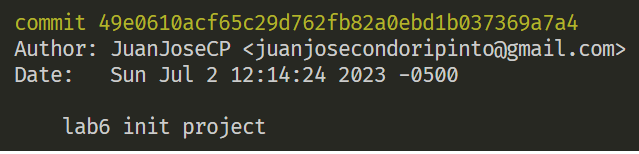
\includegraphics[width=150mm]{img/commit1.png}
        \caption{Commit 1 proyecto incial}
        \label{fig:enter-label}
    \end{figure}
    \begin{figure}
        \centering
        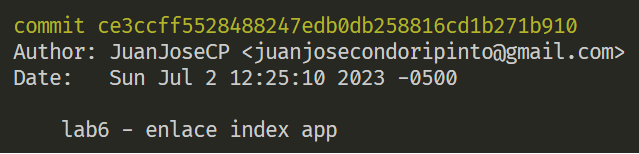
\includegraphics[width=150mm]{img/commit2.png}
        \caption{Commit 2 aqui se enlaza la aplicacion con el proyecto}
        \label{fig:enter-label}
    \end{figure}
    \begin{figure}
        \centering
        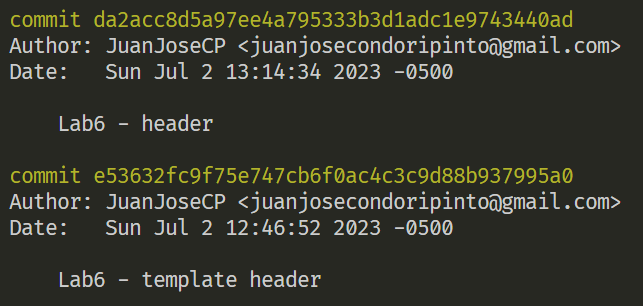
\includegraphics[width=150mm]{img/commit3.png}
        \caption{Commit 3 y 4 Creacion de la plantilla del header}
        \label{fig:enter-label}
    \end{figure}
    \begin{figure}
        \centering
        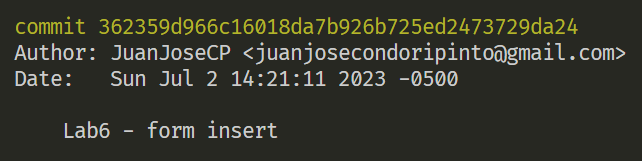
\includegraphics[width=150mm]{img/commit4.png}
        \caption{Commit 5 creacion de formulario de registro}
        \label{fig:enter-label}
    \end{figure}
    \begin{figure}
        \centering
        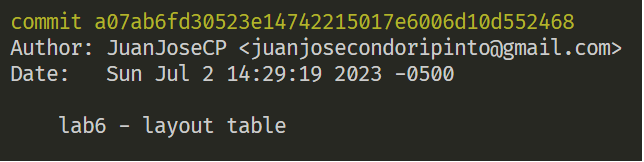
\includegraphics[width=150mm]{img/commit5.png}
        \caption{Commit 6 layout de tabla de destinos turisticos}
        \label{fig:enter-label}
    \end{figure}
    \begin{figure}
        \centering
        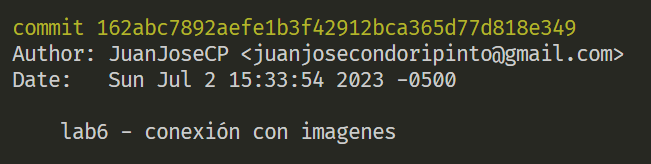
\includegraphics[width=150mm]{img/commit7.png}
        \caption{Commit 7 conexion de formulario con imagenes}
        \label{fig:enter-label}
    \end{figure}
    \begin{figure}
        \centering
        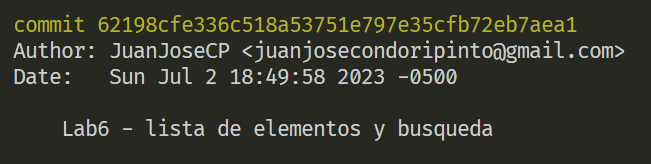
\includegraphics[width=150mm]{img/commit8.png}
        \caption{Commit 8 campo search y listado de elementos}
        \label{fig:enter-label}
    \end{figure}
    \begin{figure}
        \centering
        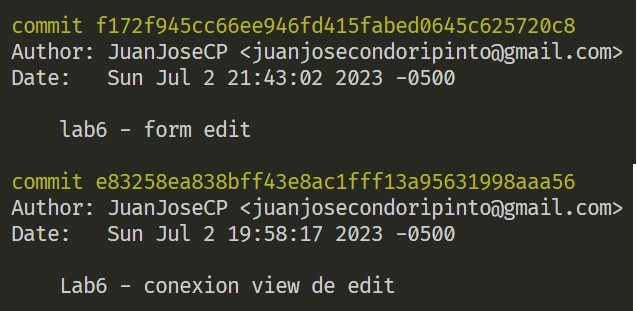
\includegraphics[width=150mm]{img/commit9.png}
        \caption{Commit 9 y 10 Formulario de edicion y conexion con view edit}
        \label{fig:enter-label}
    \end{figure}
    \begin{figure}
        \centering
        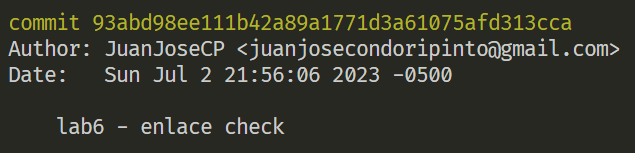
\includegraphics[width=150mm]{img/commit10.png}
        \caption{Commit 11 enlace con campo check a formulario de edicion}
        \label{fig:enter-label}
    \end{figure}
    \begin{figure}
        \centering
        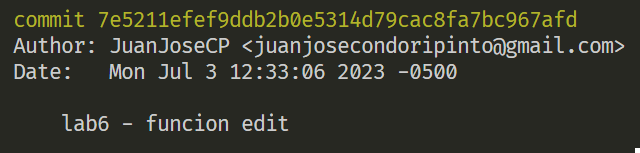
\includegraphics[width=150mm]{img/commit11.png}
        \caption{Commit 12 funcion de edicion en app}
        \label{fig:enter-label}
    \end{figure}
    \begin{figure}
        \centering
        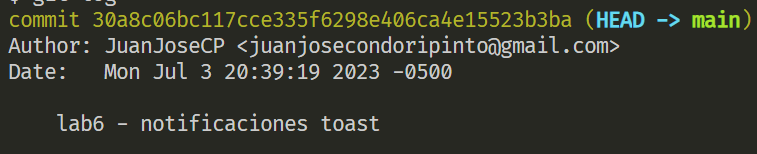
\includegraphics[width=150mm]{img/commit12.png}
        \caption{Commit 13 notificaciones con componente toast bootstrap}
        \label{fig:enter-label}
    \end{figure}

        
\section{Proyecto creado}
        \begin{figure}
            \centering
            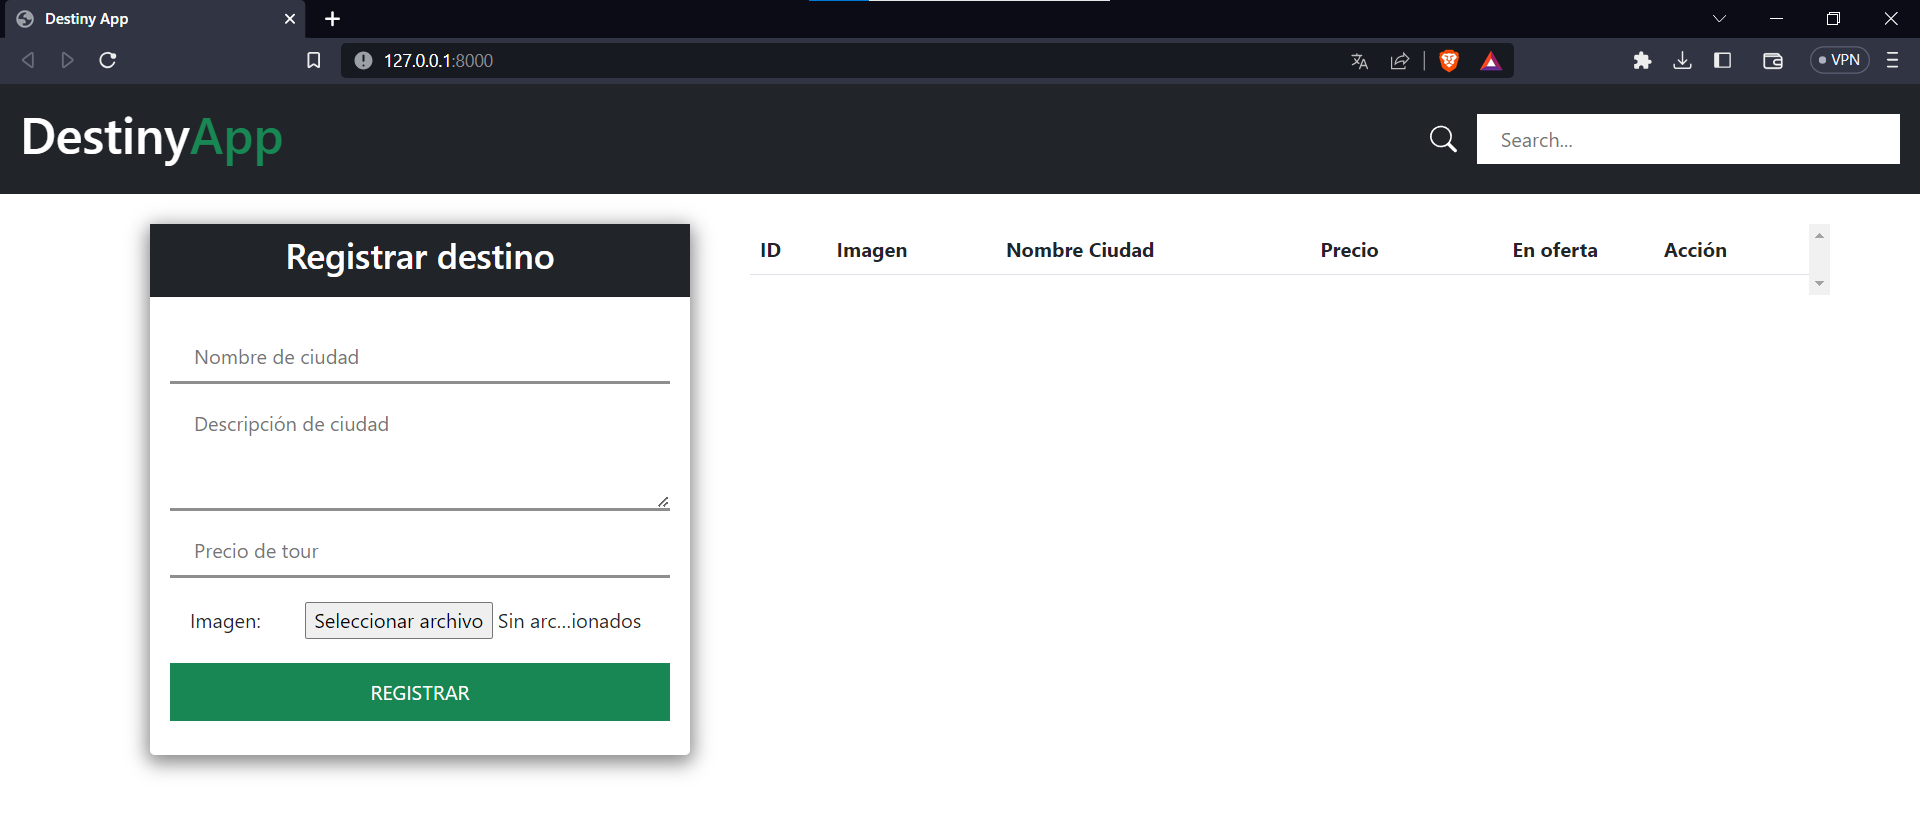
\includegraphics[width=150mm]{img/img0.png}
            \caption{Plantilla final (creacion propia)}
            \label{fig:enter-label}
        \end{figure}

        Plantilla inicial creada propiamente, usando bootstrap
        
        \begin{figure}
            \centering
            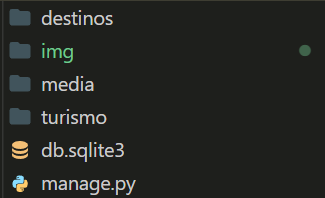
\includegraphics[width=150mm]{img/img1.png}
            \caption{Estructura de proyecto}
            \label{fig:enter-label}
        \end{figure}

        Estructura del proyecto, solo una aplicacion y media/ se usara para guardar las imagenes subidas por el cliente

        \begin{figure}
            \centering
            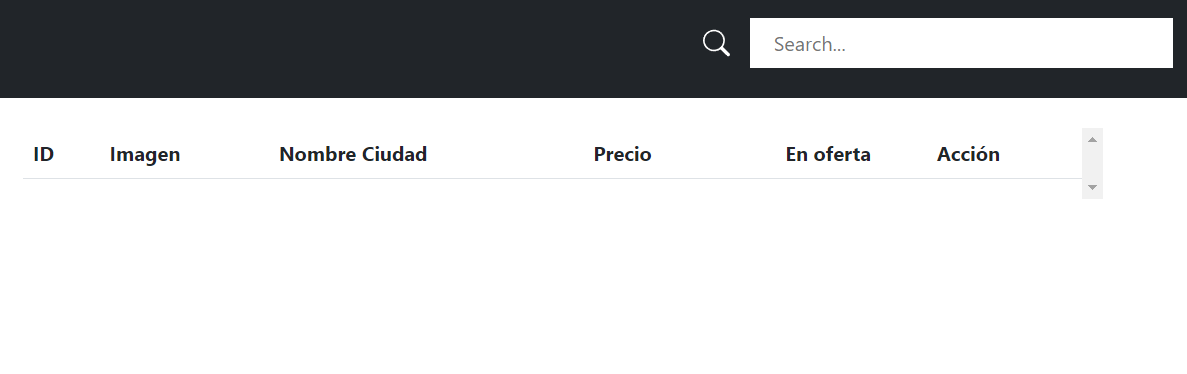
\includegraphics[width=150mm]{img/img2.png}
            \caption{Campo de busqueda y tabla}
            \label{fig:enter-label}
        \end{figure}

        Campo search de busqueda y tabla de elementos
        
        \begin{figure}
            \centering
            
\includegraphics[width=150mm]{img/img3.png}
            \caption{Formulario de registro de destino turistico}
            \label{fig:enter-label}
        \end{figure}
        
        \begin{figure}
            \centering
            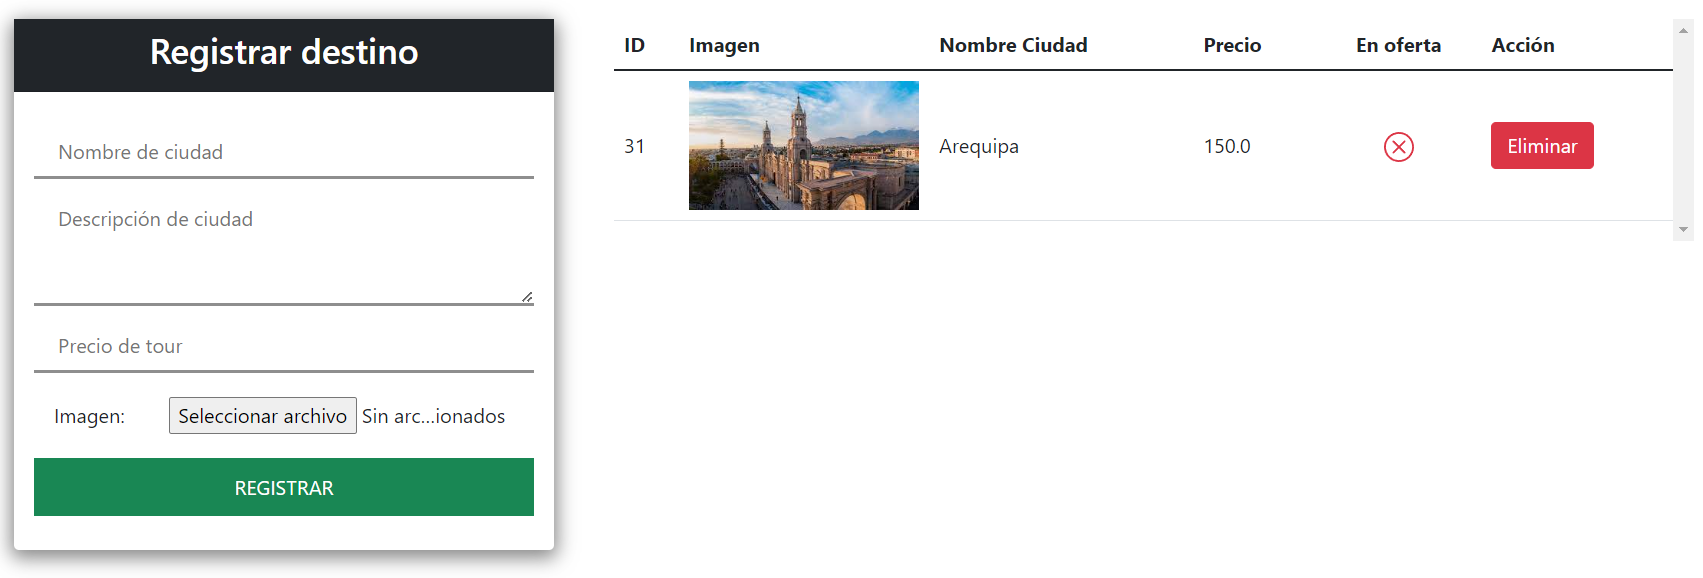
\includegraphics[width=150mm]{img/img4.png}
            \caption{Primer destino turistico registrado}
            \label{fig:enter-label}
        \end{figure}
        
        \begin{figure}
            \centering
            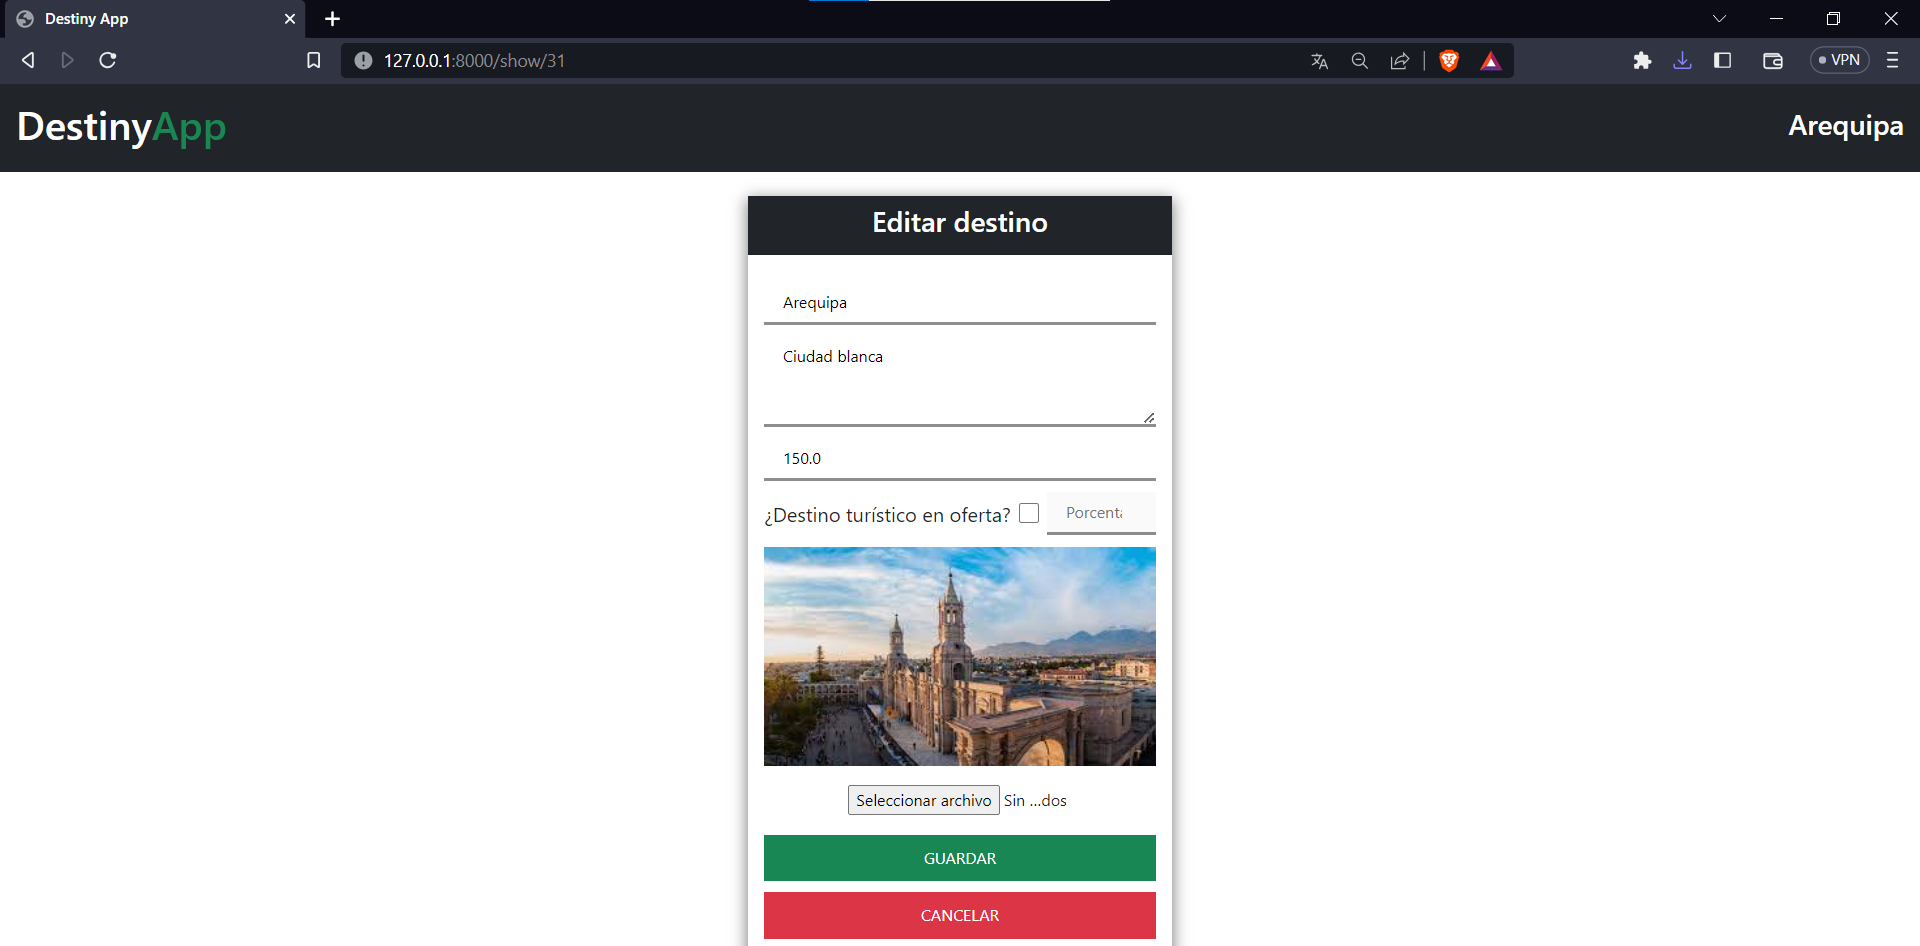
\includegraphics[width=150mm]{img/img5.png}
            \caption{Edicion de destino turistico}
            \label{fig:enter-label}
        \end{figure}
        
        \begin{figure}
            \centering
            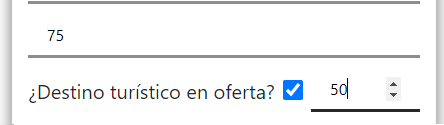
\includegraphics[width=150mm]{img/img6.png}
            \caption{Enlace entre oferta y descuento}
            \label{fig:enter-label}
        \end{figure}
        Note que aqui el descuento se contabiliza como porcentaje y se va restando automaticamente en el precio
        \begin{figure}
            \centering
            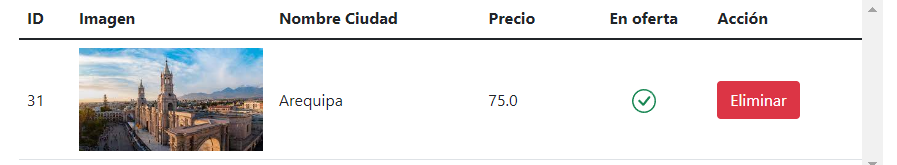
\includegraphics[width=150mm]{img/img7.png}
            \caption{Enlace con campo check de oferta}
            \label{fig:enter-label}
        \end{figure}
        
        La actualizacion funciona ya que el campo de oferta se coloca en check
        
        \begin{figure}
            \centering
            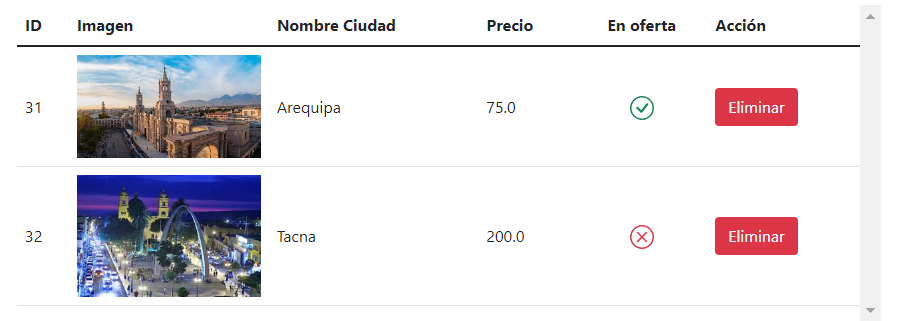
\includegraphics[width=150mm]{img/img8.png}
            \caption{Segundo destino turistico registrado}
            \label{fig:enter-label}
        \end{figure}
        
        \begin{figure}
            \centering
            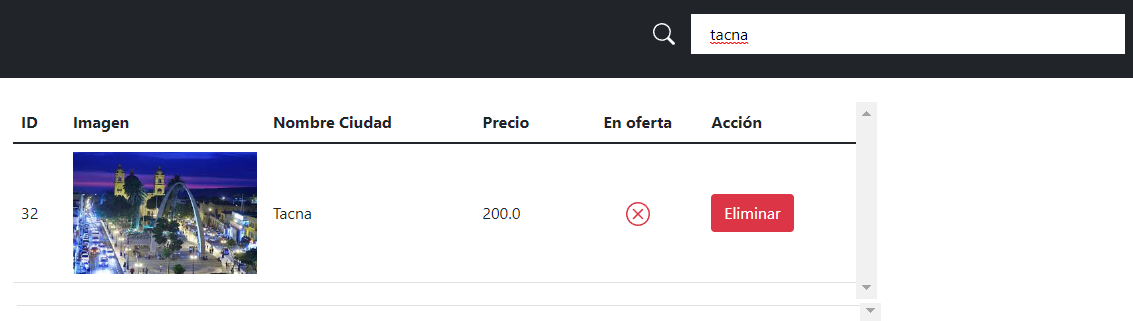
\includegraphics[width=150mm]{img/img9.png}
            \caption{Prueba de busqueda}
            \label{fig:enter-label}
        \end{figure}
        
        La busqueda se realiza cada vez que se inserta un texto en el input
        
        \begin{figure}
            \centering
            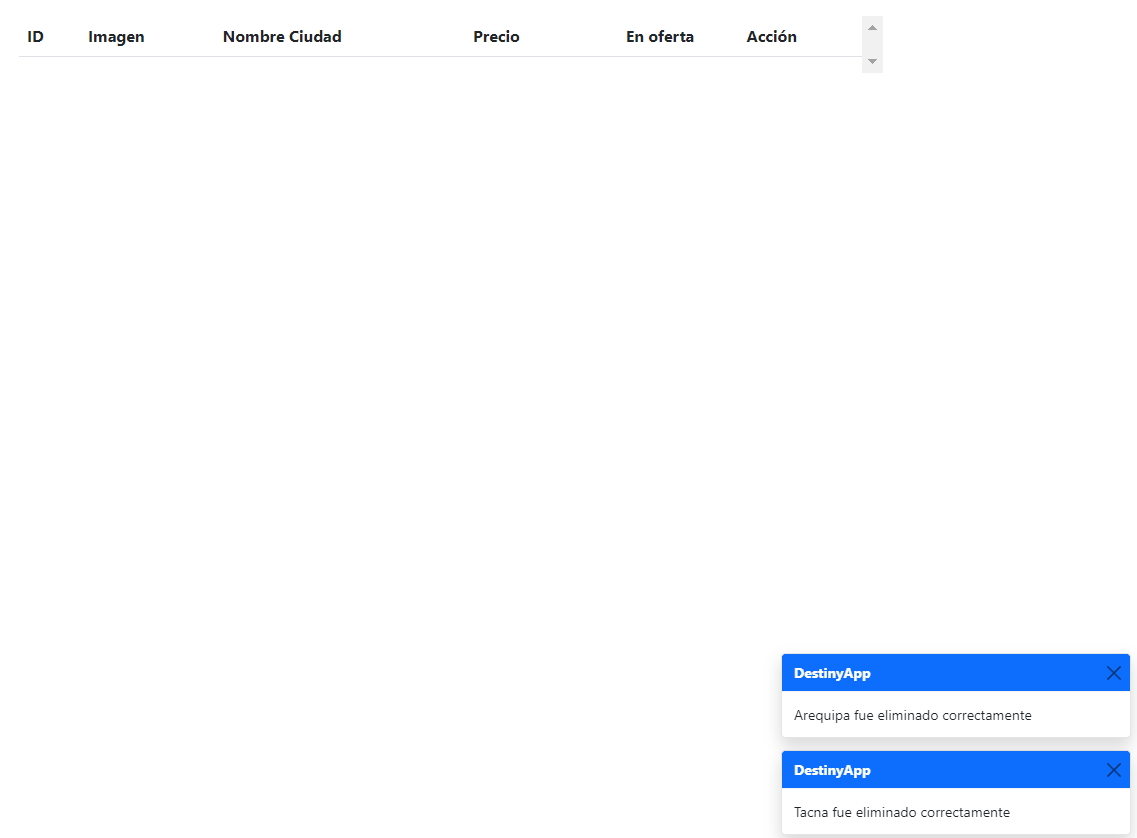
\includegraphics[width=150mm]{img/img10.png}
            \caption{Notificaciones de confirmacion de eliminacion}
            \label{fig:enter-label}
        \end{figure}
        
        Cada vez que se elimina un row aparece una notificacion que confirma dicha eliminacion y se actualiza automaticamente la tabla

        
\section{Codigo}
        \begin{lstlisting}[caption={Archivo urls.py}, label={codigo-urlsglobal}]
        # Urls general
        from django.contrib import admin
        from django.urls import path, include
        
        urlpatterns = [
            path('admin/', admin.site.urls),
            path('', include('destinos.urls'))
        ]
        
        from django.conf import settings
        from django.conf.urls.static import static
        
        if settings.DEBUG:
            urlpatterns += static(settings.MEDIA_URL, document_root=settings.MEDIA_ROOT) # Guardado de archivos media
        \end{lstlisting}

        \begin{lstlisting}[caption={Archivo urls.py de app}, label={codigo-urls}]
        from django.urls import path
        from . import views
        # rutas para app destinos turisticos
        urlpatterns = [
            path('', views.index, name='index'), # index
            path('create', views.create, name='create'),
            path('show/<id>', views.show, name='show'),
            path('edit', views.edit, name='edit'),
            path('delete/<id>', views.delete, name='delete')
        ]
        \end{lstlisting}
        
        \begin{lstlisting}[caption={Archivo models.py de app}, label={codigo-modelos}]
        from django.db import models
        
        # Create your models here.
        class Destino(models.Model):
        
            nombre = models.TextField(blank=False, unique=True, null=False, help_text="Nombre de esta ciudad de destino turístico", max_length=50)
        
            descripcion = models.TextField(blank=False, null=False, help_text="Descripción de esta ciudad de destino turístico")
        
            imagen = models.ImageField(upload_to="destinos", help_text="Imagen de esta ciudad de destino turístico")
        
            precioTour = models.FloatField(blank=False, null=False, help_text="Precio del tour a esta ciudad de destino turístico")
        
            oferta = models.BooleanField(default=False, help_text="Decide si el viaje a este destino turístico está de oferta")
        
            descuento = models.IntegerField(default=0, blank=True, help_text="Descuento establecido por oferta (porcentaje 0 - 100)")
        \end{lstlisting}
        
        \begin{lstlisting}[caption={Archivo views.py de app}, label={codigo-vistas-controladores}]
        from django.shortcuts import render, redirect
        from django.http import HttpResponse, JsonResponse, HttpResponseNotFound
        from .models import Destino
        
        # Create your views here.
        def index(request):
        
            # Consulta de todos los registros
            destinos = Destino.objects.all()
        
            return render(request, 'index.html', context={'destinos': destinos})
        
        def create(request):
        
            if request.method == 'POST':
                newDestino = Destino()
        
                newDestino.nombre = request.POST.get('nombre')
                newDestino.descripcion = request.POST.get('descripcion')
                newDestino.precioTour = request.POST.get('precioTour')
        
                newDestino.imagen = request.FILES.get('imagen')
        
                newDestino.save()
        
            return redirect('index')
        
        def delete(request, id):
        
            if request.method == 'DELETE':
                try:
                    destino = Destino.objects.get(pk=id)
        
                    nombre = destino.nombre
        
                    destino.delete()
        
                    return HttpResponse(f'{nombre} fue eliminado correctamente')
                except Exception:
                    return HttpResponseNotFound(f'Id {id} no encontrado')
            else:
                return redirect('index')
        
        
        def show(request, id):
            try:
        
                destino = Destino.objects.get(pk=id)
        
                return render(request, 'index.html', context={'destino': destino})
            
            except Destino.DoesNotExist:
        
                return redirect('index')
        
        def edit(request):
        
            try:
        
                destino = Destino.objects.get(pk=request.POST.get('id'))
                
                destino.nombre = request.POST.get('nombre')
                destino.descripcion = request.POST.get('descripcion')
                destino.precioTour = request.POST.get('precioTour')
                destino.oferta = True if request.POST.get('oferta') else False
        
                if request.POST.get('oferta'):
                    
                    destino.descuento = 0 if request.POST.get('descuento') == '' else request.POST.get('descuento')
        
                if request.FILES.get('imagen') is not None:
        
                    destino.imagen = request.FILES.get('imagen')
                
                destino.save()
        
                return redirect('index')
                
            except Destino.DoesNotExist:
        
                return redirect('index')

        \end{lstlisting}

        \begin{lstlisting}[caption={script search}, label={codigo-scripts}]
            function search() {
                let input = document.getElementById('inputSearch').value;
                
                let rows = Array.from(document.getElementsByClassName('trow'));
            
                rows.forEach(row => {
                    let nameCity = row.childNodes.item(5).textContent;
                    if (nameCity.toLowerCase().includes(input.toLowerCase())) {
                        row.style.display = ''; 
                    } else {
                        row.style.display = 'none';
                    }
                })
            }
        \end{lstlisting}

        Esta funcion de javascript es llamada cada vez que se reliza un input al campo de busqueda del header, obtiene el valor e itera en cada una de las filas de la tabla, si el campo de nombre contiene un string con el input este es mostrado, caso contrario, se oculta (no se borra)

        \begin{lstlisting}[caption={script changeEdit}, label={codigo-scripts}]
            function changeEdit(row) {
                let id = row.childNodes.item(1).textContent;
                window.location.pathname = `/show/${id}`;
            }
        \end{lstlisting}

        Esta funcion cambia la ruta actual y redirecciona a la edicion de un destino turistico, consulta segun el id

        \begin{lstlisting}[caption={script delete}, label={codigo-scripts}]
        function deleteDestiny(e) {
            e.stopPropagation();
            let row = e.target.parentNode.parentNode;
            let id = row.childNodes[1].textContent;
            let token = document.querySelector('#token').value;
            fetch(`/delete/${id}`, { 
                method: 'DELETE',
                headers: {
                    'X-CSRFToken': token
                }
            })
            .then(res => res.text())
            .then(data => {
        
                row.remove();
        
                // Crear el elemento del toast
                const toast = document.createElement('div');
                toast.classList.add('toast');
                toast.classList.add('show');
                toast.setAttribute('role', 'alert');
                toast.setAttribute('aria-live', 'assertive');
                toast.setAttribute('aria-atomic', 'true');
                toast.setAttribute('data-bs-autohide', 'true');
                toast.setAttribute('data-bs-delay', '3000');
        
                // Crear el encabezado del toast
                const toastHeader = document.createElement('div');
                toastHeader.classList.add('toast-header');
                toastHeader.classList.add('bg-primary');
                toast.appendChild(toastHeader);
        
                // Agregar el título al encabezado
                const title = document.createElement('strong');
                title.classList.add('me-auto');
                title.classList.add('text-white');
                title.textContent = 'DestinyApp';
                toastHeader.appendChild(title);
        
                // Agregar el botón de cierre al encabezado
                const closeButton = document.createElement('button');
                closeButton.setAttribute('type', 'button');
                closeButton.classList.add('btn-close');
                closeButton.setAttribute('data-bs-dismiss', 'toast');
                closeButton.setAttribute('aria-label', 'Cerrar');
                toastHeader.appendChild(closeButton);
        
                // Agregar el contenido al cuerpo del toast
                const toastBody = document.createElement('div');
                toastBody.classList.add('toast-body');
                toastBody.textContent = data;
                toast.appendChild(toastBody);
        
                // Agregar el toast al contenedor
                const toastContainer = document.getElementById('toast-container');
                toastContainer.appendChild(toast);
        
                // Mostrar el toast
                const bsToast = new bootstrap.Toast(toast, { autohide: true, delay: 3300 });
                bsToast.show();
        
                toast.addEventListener('hidden.bs.toast', () => {
                    toast.remove();
                });
            })
            .catch(err => {
                // Crear el elemento del toast
                const toast = document.createElement('div');
                toast.classList.add('toast');
                toast.classList.add('show');
                toast.setAttribute('role', 'alert');
                toast.setAttribute('aria-live', 'assertive');
                toast.setAttribute('aria-atomic', 'true');
                toast.setAttribute('data-bs-autohide', 'true');
                toast.setAttribute('data-bs-delay', '3000');
        
                // Crear el encabezado del toast
                const toastHeader = document.createElement('div');
                toastHeader.classList.add('toast-header');
                toastHeader.classList.add('bg-primary');
                toast.appendChild(toastHeader);
        
                // Agregar el título al encabezado
                const title = document.createElement('strong');
                title.classList.add('me-auto');
                title.classList.add('text-white');
                title.textContent = 'DestinyApp';
                toastHeader.appendChild(title);
        
                // Agregar el botón de cierre al encabezado
                const closeButton = document.createElement('button');
                closeButton.setAttribute('type', 'button');
                closeButton.classList.add('btn-close');
                closeButton.setAttribute('data-bs-dismiss', 'toast');
                closeButton.setAttribute('aria-label', 'Cerrar');
                toastHeader.appendChild(closeButton);
        
                // Agregar el contenido al cuerpo del toast
                const toastBody = document.createElement('div');
                toastBody.classList.add('toast-body');
                toastBody.textContent = err;
                toast.appendChild(toastBody);
        
                // Agregar el toast al contenedor
                const toastContainer = document.getElementById('toast-container');
                toastContainer.appendChild(toast);
        
                // Mostrar el toast
                const bsToast = new bootstrap.Toast(toast, { autohide: true, delay: 3300 });
                bsToast.show();
        
                toast.addEventListener('hidden.bs.toast', () => {
                    toast.remove();
                });
            });
        }
        \end{lstlisting}

        Esta funcion es llamada por medio de un evento en el boton "Eliminar" mostrado a partir de la figura 16, donde se crea un div de clase "toast" (propio de bootstra) para simular las confirmaciones en eliminacion de datos.

        \begin{lstlisting}[caption={script descuento}, label={codigo-scripts}]
        function displaySale(check) {
            let input = document.getElementById('inDescuento');
        
            if (check.checked) {
                input.removeAttribute('disabled');
            } else {
                input.setAttribute('disabled', true);
            }
        }
        
        // Para no borrar el precio inicial
        const inputPrecio = document.getElementById('precioTour'); 
        const precioInicial = inputPrecio != null ? inputPrecio.value : 0;
        function descontar() {
        
            let precio = document.getElementById('precioTour');
            let descuento = document.getElementById('inDescuento').value;
            
            precio.value = precioInicial * (1 - descuento / 100);
        
        }
        \end{lstlisting}

        La primera funcion permite habilitar el campo de descuento (input) según se haga marcado el inputcheck de oferta, la 2da funcion se llama cada vez que se inserta un valor en el campo de descuento, con la finalidad de modificar dinamicamente las ofertas, el valor inicial se guarda para evitar perdidas
    
\section{\textcolor{red}{Rubricas}}
        \subsection{\textcolor{red}{Rubrica para entregable Informe}}
            \begin{table}[ht]
                \centering
                \caption{Rúbrica para tipo de informe}
                \begin{tabular}{
                        |p{2.5cm}
                        |p{6cm}
                        |p{2cm}
                        |p{2cm} |}
                    \hline
                        \multicolumn{2}{|c|}{\textbf{Informe}} & \centerline{\textbf{Cumple}} & \centerline{\textbf{No cumple}} \\
                    \hline
                        \textbf{\textcolor{red}{Latex}} & \textcolor{blue}{El informe esta en formato PDF desde Latex, con un formato limpio (buena presentación) y facil de leer.} & \centerline{20} & \centerline{0} \\
                    \hline
                        \textbf{MarkDown} & El informe esta en formato PDF desde MarkDown README.md, con un formato limpio (buena presentacion) y facil de leer. & \centerline{17} & \centerline{0}\\
                    \hline
                        \textbf{MS Word} & El informe esta en formato PDF desde plantilla MS Word, con un formato limpio (buena presentacion) y facil de leer. & \centerline{15} & \centerline{0}\\
                    \hline
                        \textbf{Observaciones} & Por cada observacion se le descontara puntos. & \centerline{-} & \centerline{-}\\
                    \hline
                    \end{tabular}
                \label{tab:tab1}
            \end{table}
        \subsection{\textcolor{red}{Rubrica para el contenido del Informe y demostracion}}
            \begin{itemize}
                \item El alumno debera marcar o dejar en blanco en las celdas de la columna Checklist, deacuerdo a si cumplio o no con el ́ıtem correspondiente.
                \item Si un alumno supera la fecha de entrega, su calificacion siempre sera sobre la nota mınima aprobada, siempre y cuando cumpla con todos lo items.
                \item El alumno debe autocalificarse en la columna Estudiante de acuerdo a la tabla de calificacion de niveles de desempeño:
            \end{itemize}
            \begin{table}[ht]
                \centering
                \caption{Niveles de desempeño}
                \begin{tabular}{
                        >{\centering\arraybackslash}m{1.2cm}
                        >{\centering\arraybackslash}m{3cm}
                        >{\centering\arraybackslash}m{3cm}
                        >{\centering\arraybackslash}m{3cm}
                        >{\centering\arraybackslash}m{3cm}}
                    \hline
                    \multicolumn{5}{c}{Nivel} \\
                    \hline
                    \textbf{Puntos} & Insatisfactorio 25\% & En Proceso 50\% & Satisfactorio 75\% & Sobresaliente 100\% \\
                    \textbf{2.0} & 0.5 & 1.0 & 1.5 & 2.0 \\
                    \textbf{4.0} & 1.0 & 2.0 & 3.0 & 4.0 \\
                    \hline
                \end{tabular}
                \label{tab:tab2}
            \end{table}
            \begin{table}[]
                \centering
                \caption{Rubrica para contenido del Informe y demostracion}
                \begin{tabular}{
                    |m{2.5cm}
                    |m{7cm}
                    |>{\centering\arraybackslash}m{1cm}
                    |>{\centering\arraybackslash}m{1.2cm}
                    |>{\centering\arraybackslash}m{1.5cm}
                    |>{\centering\arraybackslash}m{1.2cm}|}
                    
                    \hline
                    \multicolumn{2}{|c|}{Contenido y demostracion} & Puntos & Checklist & Estudiante & Profesor \\
                    \hline
                    \textbf{1. GitHub} & Hay enlace URL activo del directorio para el laboratorio hacia su repositorio GitHub con codigo fuente terminado y facil de revisar. & 2 & X & 2 &   \\
                    \hline
                    \textbf{2. Commits} & Hay capturas de pantalla de los commits mas importantes con sus explicaciones detalladas. (El profesor puede preguntar para refrendar calificacion). & 4 & X & 3 &   \\
                    \hline
                    \textbf{3. Código fuente} & Hay porciones de codigo fuente importantes con numeracion y explicaciones detalladas de sus funciones. & 2 & X & 2 &   \\
                    \hline
                    \textbf{4. Ejecucion} & Se incluyen ejecuciones/pruebas del codigo fuente explicadas gradualmente. & 2 & X & 2 &   \\
                    \hline
                    \textbf{5. Pregunta} & Se responde con completitud a la pregunta formulada en la tarea. (El profesor puede preguntar para refrendar calificacion). & 2 & X & 2 &   \\
                    \hline
                    \textbf{6. Fechas} & Las fechas de modificacion del codigo fuente estan dentro de los plazos de fecha de entrega establecidos. & 2 & X & 2 &   \\
                    \hline
                    \textbf{7. Ortografia} & El documento no muestra errores ortograficos. & 2 & X & 2 &   \\
                    \hline
                    \textbf{8. Madurez} & El Informe muestra de manera general una evolucion de la madurez del codigo fuente, explicaciones puntuales pero precisas y un acabado impecable. (El profesor puede preguntar para refrendar calificacion). & 4 & X & 3 &   \\
                    \hline
                    \multicolumn{2}{|c|}{Total} & 20 &  & 18 & \\
                    \hline
                \end{tabular}
                \label{tab:tab3}
            \end{table}
    
\section{Referencias}
        \begin{itemize}
            \item \url{https://developer.mozilla.org/en-US/docs/Learn/Server-side/Django/Tutorial_local_library_website}
            \item \url{https://github.com/mdn/django-locallibrary-tutorial}
            \item \url{https://github.com/rescobedoq/pw2/tree/main/labs/lab05}
            \item William S. Vincent. (2022). Django for Beginners: Build websites with Python. Django 4.0.leanpub.com [\href{http://library.lol/main/22AF742D96697DE55EF5F88B08F1AA86}{URL}]
            \item \url{https://docs.djangoproject.com/en/4.1/ref/models/fields/}
            \item \url{https://docs.djangoproject.com/en/4.0/topics/db/examples/many_to_many/}
            \item \url{https://docs.djangoproject.com/en/4.0/topics/db/examples/many_to_one/}
            \item \url{https://blog.hackajob.co/djangos-new-database-constraints/}
            \item \url{https://stackoverflow.com/questions/3330435/is-there-an-sqlite-equivalent-to-mysqls-describe-table}
            \item \url{https://docs.djangoproject.com/en/4.1/ref/validators/#how-validators-are-run}
            \item \url{https://docs.djangoproject.com/en/4.1/ref/models/instances/}
        \end{itemize}
\end{document}  